\documentclass{article}

% Gives us lovely headers
\usepackage{fancyhdr}
% For pretty pictures
\usepackage{graphicx}
% Means you don't have to put \\ to start a new line.
\usepackage[parfill]{parskip}
% For line brakes in tables
\usepackage{tabularx}
% For the split environment
\usepackage{amsmath}
% For tabs in verbatim and the listings environment
\usepackage{moreverb}
% Gives us bigger margins on the right (and smaller on the left) for the margin
% paragraphs
\usepackage[left=2cm,
			top=3cm,
			right=5cm,
			bottom=3cm,
			marginparwidth=4cm,
			marginparsep=3mm]{geometry}

% Means that I don't have to type \marginpar{\raggedright \scriptsize every 
% time I want a margin paragraph
\makeatletter
\renewcommand{\@marginparreset}{%
  \reset@font\scriptsize
  \raggedright
  \@setminipage
}
\makeatother

% Like a quote but without the indent
\newenvironment{fancyquote}{
	\list{}{
		\leftmargin=0.3in
		\rightmargin=0.3in
	}
		\item[]
	{\endlist}
}

\begin{document}
% Meta
\author{Todd Davies}
\title{COMP12111 notes}
\rhead{COMP12111 notes}
\chead{}

\maketitle
\thispagestyle{empty}

{\small Note, extra space has been allocated for the right hand margin to allow
for more extensive margin notes. Also, it gives you space to make your own
annotations and perhaps try some problems of your own.}

\tableofcontents
\thispagestyle{empty}

\newpage
\setcounter{page}{1}

\section*{Introduction}

Unlike many of the courses, the university supplied notes for this course are of
a very high quality. This is especially true of the notes covering the first
half of the course (weeks one through six). In light of this, I've decided not
to write notes on the first half, but concentrate solely on the second half of
the course. However, it is likely that I will produce other resources such as
summary notes or flashcards for the whole of the course.

\section{The three box model}

The three box model describes the classic model of a computer. The three boxes
consist of the CPU, the memory and I/O.

\begin{figure}[ht!]
	\centering
	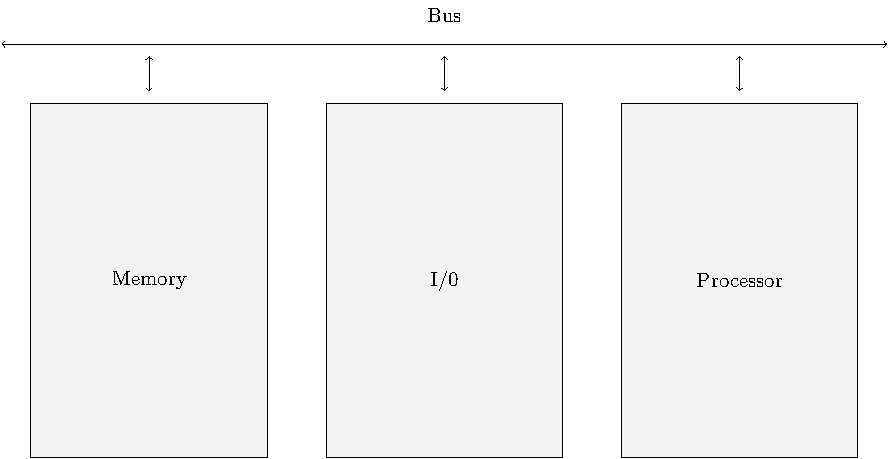
\includegraphics[width=\textwidth]{three_box_model.pdf}
	\caption{An example of the three box model}
	\label{overflow}
\end{figure}

% Take a look at the 3_box_model_description branch for info I took out from
% here

\subsection{The Amdahl/Case rule}

A computer that has one disproportionately powerful component is very wasteful
since the other components will act as a limiting factor with regard to the
speed of the computer. It's no good having a fantastically fast processor with a
tiny amount of RAM.

The Amdahl/Case rule gives us guidelines that we can use to determine sensible
specifications for components within a computer. Though there are many different
versions of this rule, it is something along the lines of:

\marginpar{MIPS stands for million instructions per second}

\begin{fancyquote}
		A balanced computer system needs about one megabyte of main memory and
		about one megabit per second of I/O per MIPS of CPU performance.
\end{fancyquote}

\subsection{CPU}

\subsubsection{The fetch, decode, execute cycle}

The CPU is essentially a large FSM\marginpar{FSM = Finite State Machine} that
loops over three operations; fetch, decode and execute in order to perform the
instructions defined in a program.

\paragraph{Fetch}\mbox{}

The processor first reads a word \marginpar{1 word = 4 bytes}from an address
that is pointed to in memory by a {\it pointer}. After the instruction has been
read, the pointer is moved on to the next address in memory.

\paragraph{Decode}\mbox{}

The instructions that are to be loaded from memory are really just a really long
list of numbers. However, each number is coded in such a way that it represents
an action. A rudimentary way of encoding such a system would be to let the
number $1$ mean 'shift bits left' and the number $2$ mean 'shift bits right'. An
operation code is obtained from the instruction and the control signals specific
to that code are then set for the FSM.

\paragraph{Execute}\mbox{}

\marginpar{A datapath is a collection of logic units to perform arithmetic or
other functions. See course supplied notes for more information on datapaths.}

In this phase, the data is moved through the datapath and the instruction that
was in memory is now performed. The processor then starts the cycle again, by
fetching an instruction from memory.

\subsubsection{Maintaining state}

A CPU is required to maintain some form of state while processing instructions,
since most instructions have interactions between one another. In order to keep
track of what's going on in between instructions, the CPU uses both the registers
that is has built in and the main memory.

It is important to realise that the whole system changes state at the same time,
driven by a central {\it clock}. This means that all the parts of the system are
in sync with each other. In fact, we can treat the system as a whole (including
the memory and registers) as a finite state machine.

\subsubsection{Address spaces}

An address space is a number of memory locations that a system can address. Each
location in memory has a unique address, which is a number.

Memory addresses are countable, i.e. you can increment one to get the next one
and decrement one to get the previous one. However, they are sometimes not
countable in the traditional sense. First of all, they are usually counted in
hexadecimal in order to save characters and enable easy conversion to binary,
with each digit converting to four bits. Second of all, the length of the word
defines the gap between each countable memory location.

\marginpar{N.b. Most processors offer the capability to address bytes in between
the words too}

For example, in 32 bit processors, words are defined as 32 bits long.
Henceforth, each memory location is contains 32 bits, and so the addresses go up
in fours. In a 64 bit processor, the gap between adjacent addressable words in
memory would be eight addresses.

The number of bits in a word is very important for a number of reasons. Longer
words usually mean longer instructions, so more information can fit inside,
meaning less instructions need to be executed to perform tasks. Also, longer
words means more addressable memory locations; in a 32 bit system, there are
$2^32$ memory locations, but in a 64 bit system, there are $2^64$ addressable
memory locations. This is why 32 bit systems are limited to 4GB or RAM.

\subsection{Memory}

Memory allows the processor to write store and load data. It is often referred
to as Random Access Memory. As opposed to hard drives, where in order to access
different locations a physical component must be moved, RAM is able to access
any location in any order with no time penalty, hence the usage of the term {\it
random}.

We can work out how many bits are required to address a memory of a given size.
In order to do this, we must find the power of 2 equal to or above the size of
the memory (in bytes), and split it into common factors (which should also be
powers of two) then we add up the powers, which will give us our number of bits.
Here are some examples:

{\bf Find the number of bits required to address 1 Kbyte of memory}

\begin{enumerate}
	\item Find the powers of two that will go into 1 Kbyte:
			1 Kybte = $2^{10}$ bytes
\end{enumerate}

{\bf Find the number of bits required to address 64M bytes of memory}

\begin{enumerate}
	\item Find the powers of two that will go into 64 Mbytes:
			64 Mybtes = $2^{26}$ bytes = $2^6 + 2^{20}$ bytes
	\item Add the powers together:
			$6 + 20 = 26$ bits
\end{enumerate}


{\bf Find the amount of memory that can be addressed by 19 bits}

\begin{enumerate}
	\item $2^{19} = 2^{10} \times 2^{9} = 1,024 \times 512 = $ 512 Kbytes
\end{enumerate}

\subsubsection{Memory caching}

A commonly used optimisation for memory is to use a cache. This is a small
amount of extra memory that is very fast to access. The values stored in memory
addresses that are being accessed frequently can be temporarily stored here
instead to avoid the comparatively slow referencing of the main memory.

\subsection{Input/Output}

IO is concerned with interfacing with peripheral devices such as keyboards,
monitors, networks etc. Each device will have an interface to a specific bus
that can communicate with memory and the CPU.

A {\it port} is a form of I/O  that is usually mapped to an area of memory. In
the eyes of the CPU, a simple output port is just an area of memory to be read
from and written to, however, it will also be mapped to some external connection
such as lights, motor or even more complicated devices such as a printer.

An input port will also 'look' like an area of memory to the CPU, however, that
area of memory will be connected to external signals.

\marginpar{Most ports are 8-bits wide, even in processors that use larger word
lengths.}

It is also possible to have bidirectional ports, however, this requires extra
coordination to ensure that reading and writing doesn't take place at the same
time.

\paragraph{Types of ports}\mbox{}

There are two main types of ports, serial and parallel. Parallel ports are as
described above; just a collection of wires that can be in the states 1 or 0. In
order to send a 1 Mbyte file over a parallel port, could either have eight
million wires or you can use only eight wires and splitting the file into one
million parts.

Serial ports only deal with single bits, and so require one wire. This may seem
very slow, but a lot of time is often spent optimising the transfer so its
speeds are comparable with parallel ports. However, serial ports often need
extra registers to signal other information such as transfer speed and the
direction of transfer.

\subsection{Buses}

A bus is a collection of signals that act together.

There are three buses used by the CPU:

\begin{itemize}
	\item {\bf Address bus}
		This is an output for the processor, and is used to specify the location
		in Memory or I/O for data to be transferred. It is usually as wide as
		the word length of the processor.
	
	\item {\bf Data bus}
		This is usually a bidirectional bus, usually as wide as a processor's
		registers (that in turn are usually as wide as a word). However, a
		smaller data bus will reduce the cost of the processor, but a larger bus
		will enable a higher bandwidth, which could let the processor fetch more
		than one instruction in one cycle!\marginpar{N.b. Another way to make a
		bus go faster is to increase the clock speed it is running at.}

	\item {\bf Control bus}
		The main function of the control bus is to specify the direction of the
		flow of data. However, it also has a lot of other functions which aren't
		relevant here.
\end{itemize}

\end{document}
